
                \begin{figure}
                    \centering
                    \begin{tikzpicture}
                        \pgfplotsset{%
                            width=1\textwidth,
                            height=0.4\textheight
                        }
                        \begin{axis}[
                            xlabel={Start temperature},
                            ylabel={Average dynamic energy (watt)},
                            ymin=0,ymax=100,
                        ]
                        
                            \addplot [mark=none, densely dashed, red]  coordinates {
                            (35, 0.020960547325840212)(40, 0.02037215780598898)(45, 0.01897032839726835)
                            };
                            \addlegendentry{WRK - IPG}
                            
                            \addplot [mark=none, densely dashed, blue]  coordinates {
                            (35, 0.06582153891630892)(40, 0.022483607348426634)(45, 0.023437932226106364)(50, 0.020434628037683904)
                            };
                            \addlegendentry{WRK - LHM}
                            
                            \addplot [mark=none, densely dashed, cyan]  coordinates {
                            (40, 0.0)(45, 0.0)(60, 0.0)
                            };
                            \addlegendentry{WRK - CLAMP (win)}
                            
                        \end{axis}
                    \end{tikzpicture} 
                \caption{A graph illustrating the energy consumption of Dram for test case Fasta with regards to the temperature of the DUT, experiment \#2, (without outliers)} \label{fig:Fasta_Dram_temperature_exp2}
                \end{figure}
                